% ========================================================================================
%	Question 1
% ========================================================================================

\section{Part A}

\subsection{Write a RISC-V assembly program for multiplication}
\textbf{Description: Write a RISC-V assembly program to compute the product of two integer values. The two values should be initialized in main(). The main() function should call the product(int x, int y) function, passing the two integer values as arguments. The product function should return the product of the two numbers.}
\subsubsection{Develop both a non-recursive and recursive implementation of your assembly program. Submit your assembly code on Blackboard through Turnitin.}
\subsubsection{What is the largest product that can be computed in your program?}
\subsubsection{Discuss how you implemented integer multiplication, since it is not directly supported on the simulator. Discuss an alternative implementation for multiplication. Which implementation would you expect to perform better, and why?}

\subsection{Write a recursive RISC-V assembly program to compute the factorial}
\textbf{Description: Write a recursive RISC-V assembly program to compute the factorial of a value that is initialized in main (). We provide a recursive factorial program in the c program example on Blackboard.}
\subsubsection{Submit your assembly code on Blackboard through Turnitin.}

\subsection{What is the largest integer value for factorial}
\textbf{Description: What is the largest integer value that you can compute the factorial in your program on the RV32I ISA? Explain why.}

\breakrule

\subsection{Solution}

% Sample text
This is where you write your answers. Adding a figure as an example. You can reference it using this: Figure ~\ref{fig:example}.

\begin{figure}[!htbp]
\centering 
        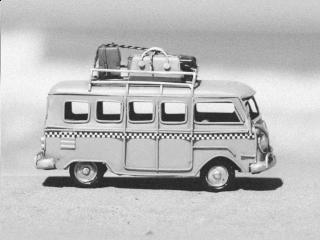
\includegraphics[width=0.3\textwidth]{figs/beachbus.jpg}
        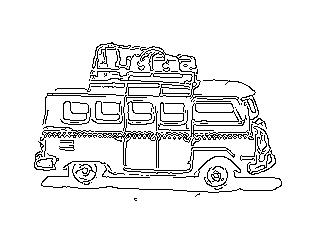
\includegraphics[width=0.3\textwidth]{figs/beachbus-canny.jpg}
\caption[Original image and post processed image]{Original image (A) and post-processed image (B).}
\label{fig:example} 
\end{figure}

You should add a copy of your code in the homework report as well:

\begin{lstlisting}[language=Python, caption=Python example]
import numpy as np
 
def incmatrix(genl1,genl2):
    m = len(genl1)
    n = len(genl2)
    M = None #to become the incidence matrix
    VT = np.zeros((n*m,1), int)  #dummy variable
 
    #compute the bitwise xor matrix
    M1 = bitxormatrix(genl1)
    M2 = np.triu(bitxormatrix(genl2),1) 
 
    for i in range(m-1):
        for j in range(i+1, m):
            [r,c] = np.where(M2 == M1[i,j])
            for k in range(len(r)):
                VT[(i)*n + r[k]] = 1;
                VT[(i)*n + c[k]] = 1;
                VT[(j)*n + r[k]] = 1;
                VT[(j)*n + c[k]] = 1;
 
                if M is None:
                    M = np.copy(VT)
                else:
                    M = np.concatenate((M, VT), 1)
 
                VT = np.zeros((n*m,1), int)
 
    return M
\end{lstlisting}

\newpage

% ----------------------------
% Section ends
% ============================

% ========================================================================================
%	Question 2
% ========================================================================================

\section{Part B}

\subsection{Profile Quick-sort}
\textbf{Description: For	this	problem	you	will	use	the	qsort.c	(quicksort)	program	provided,	and	you	
need	to	produce	a	dynamic	instruction	mix	table	(similar	to	Figure	A.29 in	your	
textbook)	to characterize	the	execution	of	the	quicksort	program. You	can	perform	
this	study	on	any	architecture	of	your	choice.	There	are	a	number	of approaches	you	
can	take	to	produce	this	data. Please	make	sure	to	explain	how	you	produced	the	data	in	your	table	and	provide
details	of	the	tools	that	you	used.}
\subsubsection{You	could	instrument	the	code	to	capture	the	execution	frequency	of	each
basic	block,	and	then,	using	an	assembly	listing	of	the	program,	provide
instruction	counts	(this	is	slightly	imprecise,	but	very	acceptable	for	this
assignment).}
\subsubsection{You	could	find	a	tracing	program	that	can	capture	an	instruction	trace.	You
would	then	have	to	write	a	program	to	count	individual	instructions
(challenging,	but	not	impossible).}
\subsubsection{You	could	find	a	tool	out	on	the	Internet	that	provides	this	capability	already
for	you.	While	this	sounds	easy,	it	may	be	a	bit	of	work	to	learn	the	particular
tool	you	have	chosen	to	use.}

\breakrule

\subsection{Solution}

% Sample text
This is where you write your answers. Adding a table as an example. You can reference it using this: Table~\ref{tab:example}.

\begin{table}[!htbp]
  \begin{center}
    \caption{Your first table.}
    \label{tab:example}
    \begin{tabular}{l|c|r} % <-- Alignments: 1st column left, 2nd middle and 3rd right, with vertical lines in between
      \textbf{Value 1} & \textbf{Value 2} & \textbf{Value 3}\\
      $\alpha$ & $\beta$ & $\gamma$ \\
      \hline
      1 & 1110.1 & a\\
      2 & 10.1 & b\\
      3 & 23.113231 & c\\
    \end{tabular}
  \end{center}
\end{table}

Adding a reference. The references are all in bib format. You can obtain these references from google scholar. Makes it a lot easier to add the references you need to cite on the homework. Just search for the paper you were reading on google scholar, and click on cite and search for the bibtex format. Add this reference (text) into the bib/sample.bib file and then cite the reference name inside this code. An example: Using the book~\cite{book} we answer the questions by providing Table~\ref{tab:example}. Tables can be generated with:
\lstinline{https://www.tablesgenerator.com/}.


\newpage

% ----------------------------
% Section ends
% ============================

% ========================================================================================
%	Question 3
% ========================================================================================

\section{Part C}

\subsection{Floating point benchmarks}
\textbf{Description: For	this	part	of	the	assignment,	write	two	different	benchmark	programs	on	your	
own that	contain significant	floating-point	content.		Compile	the	programs on	X86	
and	generate	an	assembly	listing	of the	benchmarks.		Then	identify	4 different	
floating-point	instructions	used	in	each program (a	total	of	8) and	explain	both	the	
operands	used	by	each	instruction	and	the	operation performed	on	the	operands	by	
the	instruction.}

\breakrule

\subsection{Solution}

\newpage

% ----------------------------
% Section ends
% ============================

% ========================================================================================
%	Question 4
% ========================================================================================

\section{Part D}

\subsection{Appendix K}
\textbf{Description: For	this	problem	you	will	need	to	read	through	Appendix	K	in	your	text,	covering	a	
number	of	instructions	sets,	and	then	answer	the	following	questions:}
\subsubsection{Name	2	CISC	instruction	set	architectures	and	2	RISC	instruction	set	
architectures.}
\subsubsection{Describe	3	characteristics	of	the	DEC	Alpha instruction	set.}
\subsubsection{Discuss	the	differences/similarities	between	MIPS	and	PowerPC	in	terms	of	
how	they	handle	conditional	branches.}
\subsubsection{Given	an	example	of	how	register	windows	work	on	the	SPARC	ISA.}
\subsubsection{In	your	opinion,	which	generation	of	the	Intel	x86	architecture	was	the	most	
significant	advancement	from	the	previous	generation	of	the	ISA.}

\breakrule

\subsection{Solution}


\newpage

% ----------------------------
% Section ends
% ============================

% ========================================================================================
%	Question 4
% ========================================================================================

\section{Part E}

\subsection{Amdahl}
\textbf{Description: Read	the	Amdahl,	Blaauw	and	Brooks	1964	paper	on	the	IBM	360	Architecture.
Given	the	timeframe	of	the	paper,	what	do	you	find	the	most	impressive	feature	of	
the	architecture	as	described	by	the	authors?		Justify	why	you	feel	this	is	such	a	
great	feature.		Also,	discuss the	representation	of	the	various	data types	supported	
on	this	important	ISA,	and	contrast	it	with	the	RISC-V.}

\breakrule

\subsection{Solution}


\newpage

% ----------------------------
% Section ends
% ============================

% ========================================================================================
%	Question 4
% ========================================================================================

\section{Part F}

\subsection{Chapter 1 Problems (Extra credit)}
\textbf{Description: Complete	problems	1.7,	1.8,	1.10,	and	1.12	(only	a	and	b) from	the	text.}

\breakrule

\subsection{Solution}


\newpage

% ----------------------------
% Section ends
% ============================
